\begin{figure}[t]
\centering
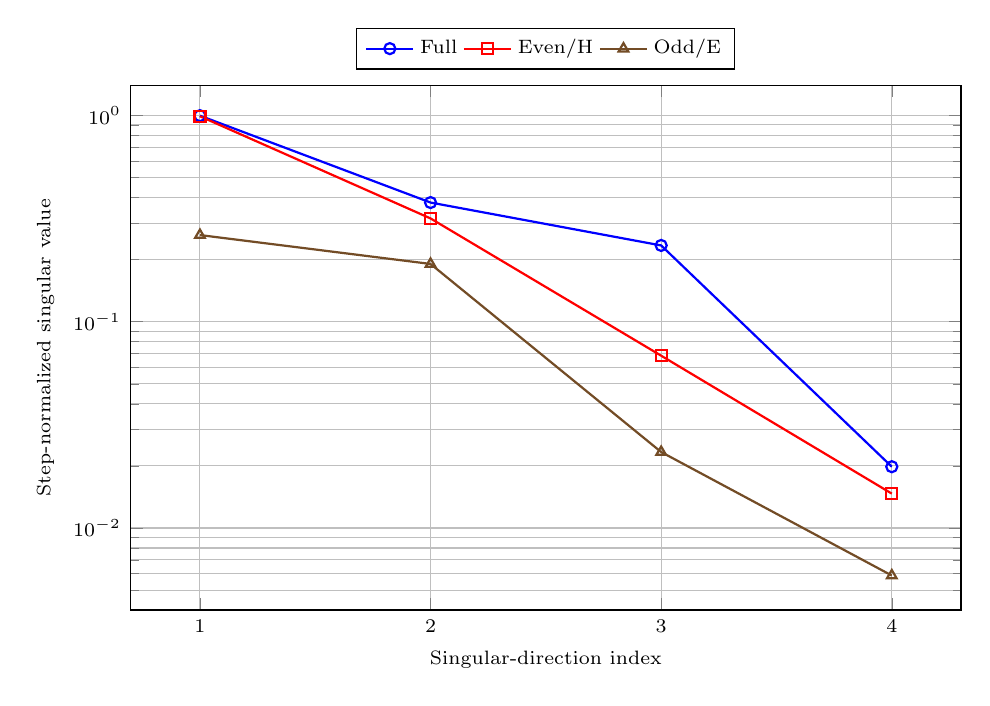
\begin{tikzpicture}
\begin{axis}[
width=\columnwidth,
height=0.68\columnwidth,
ymode=log,
ymin=0.004,
ymax=1.4,
xlabel={Singular-direction index},
ylabel={Step-normalized singular value},
xtick={1,2,3,4},
grid=both,
minor y tick num=1,
legend style={font=\scriptsize,at={(0.5,1.03)},anchor=south,legend columns=3},
tick label style={font=\scriptsize},
label style={font=\scriptsize},
]
\addplot+[mark=o,thick] coordinates {
(1,0.9978866) (2,0.3783362) (3,0.2343354) (4,0.0198217)
};
\addplot+[mark=square,thick] coordinates {
(1,0.9913428) (2,0.3168661) (3,0.0684416) (4,0.0146756)
};
\addplot+[mark=triangle,thick] coordinates {
(1,0.2631486) (2,0.1906064) (3,0.0233484) (4,0.00588186)
};
\legend{Full,Even/H,Odd/E}
\end{axis}
\end{tikzpicture}
\caption{Step-normalized singular spectra of the complete full-band Jacobian and its two parity blocks. The response space contains several strong directions together with one weak combination; the latter is a cancellation-dominated parameter combination rather than a collapse of the entire modal-control space.}
\label{fig:singular-spectrum}
\end{figure}
